% id: 0625
% book: RPM 중3-2 수학 · 06 상관관계
% section: 유형 03 산점도의 이해 (1)
% figure: crop:fig-0625.png
% answer: ⑤
% answer_source: 답지
% variant_level: 0 (원본 전사)
% 이 파일은 build.mjs 가 items.json 에서 만든다. 고칠 때는 items.json 을 고친다.
\noindent\begin{minipage}[t]{0.58\linewidth}\vspace{0pt}\raggedright 오른쪽 그림은 시하네 반 학생들의 멀리뛰기 실기 점수와 높이뛰기 실기 점수에 대한 산점도이다. 다음 중 옳지 \underline{않은} 것은?\end{minipage}\hfill\begin{minipage}[t]{0.4\linewidth}\vspace{0pt}\centering \setlength{\dmfigw}{88.2pt}\ifdim\dmfigw>\linewidth\setlength{\dmfigw}{\linewidth}\fi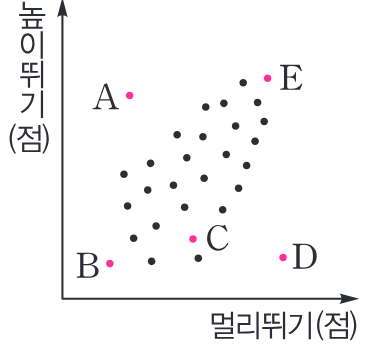
\includegraphics[width=\dmfigw]{figures/fig-0625.png}\end{minipage}\par
\par\medskip\par\noindent\hangindent=1.4em\hangafter=1 {\small ①}\ $\pt{E}$는 두 종목 모두 점수가 높은 편이다.\par\noindent\hangindent=1.4em\hangafter=1 {\small ②}\ 높이뛰기 실기 점수에 비해 멀리뛰기 실기 점수가 가장 높은 학생은 $\pt{D}$이다.\par\noindent\hangindent=1.4em\hangafter=1 {\small ③}\ 멀리뛰기 실기 점수와 높이뛰기 실기 점수 사이에는 양의 상관관계가 있다.\par\noindent\hangindent=1.4em\hangafter=1 {\small ④}\ $\pt{A}$는 멀리뛰기 실기 점수에 비해 높이뛰기 실기 점수가 높다.\par\noindent\hangindent=1.4em\hangafter=1 {\small ⑤}\ $\pt{C}$보다 $\pt{B}$가 두 종목의 실기 점수의 평균이 높다.\par\medskip
